\section{Nombre: Jaguar}   \label{per:jaguar}
\subsection{Descripción:}
Animal felino carnívoro, de color amarillo a café rojizo con manchas negras.
\subsection{Status:}
NPC, enemigo.
\subsection{Imagen}
Ver figura \ref{fig:jaguar}.
\begin{figure}
	\centering
	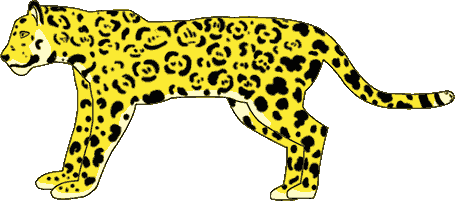
\includegraphics[height=0.2 \textheight]{Imagenes/jaguar}
	\caption{Jaguar.}
	\label{fig:jaguar}
\end{figure}
\subsection{Encuentro:}
En el nivel 8.
\subsection{Habilidades:}
\begin{itemize}
	\item Zarpazo. Ver en \ref{hab.zarpazo}.
\end{itemize}
\subsection{Patrón de ataque:}
El felino va de un lado hacia otro en dirección horizontal, cuando se encuentra con el jugador tira un zarpazo.